\Appendix


Этот элемент структуры работы не является обязательным. Приложения целесообразно вводить, когда автор использует относительно большое количество громоздких таблиц, статистического материала. Такой материал, помещенный в основную часть, затруднил бы чтение работы. Обычно в тексте достаточно лишь сослаться на подобную информацию, включенную в приложение.



\begin{table}[H]
	\caption{Такая таблица по ГОСТу}
	\label{tab:GOST3}
	\begin{center}
		\begin{tabular}{|c|c|c|}
			\hline
			\multirow{3}{*}{Размеры нестандартных болтов} & \multicolumn{2}{c|}{Диаметр} \\
			\cline{2-3}
			& Норма & Разброс \\
			\cline{2-3}
			& 10 мм & 1 мм \\
			\hline
		\end{tabular}
	\end{center}
\end{table}
Ссылка на таблицу в Приложении: Таблица~\ref{tab:GOST3}

\begin{figure}[h]
	\centering
	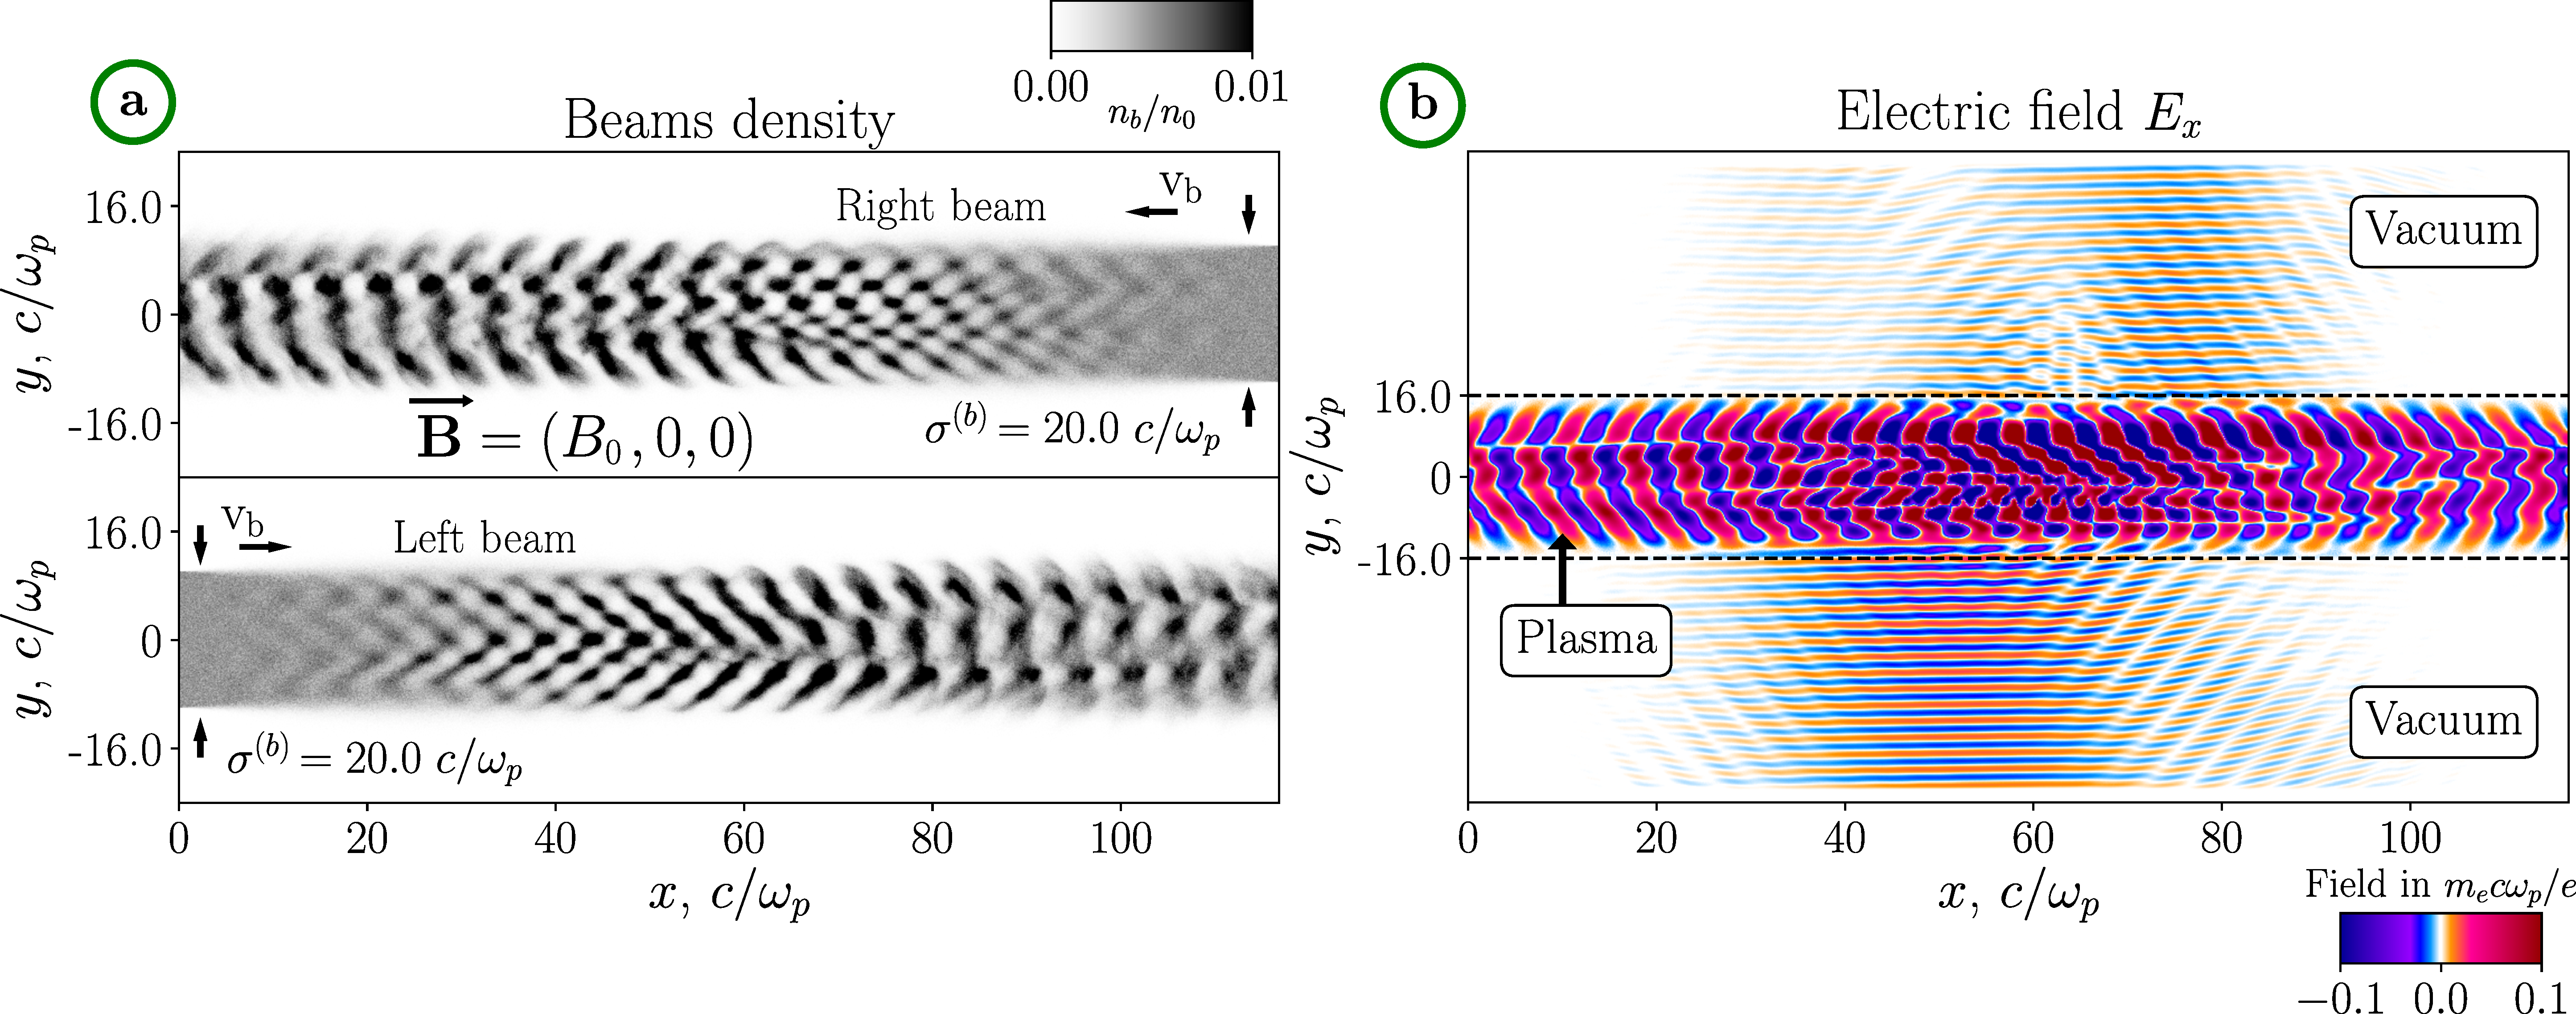
\includegraphics[width=0.45\linewidth]{fig2.pdf}
	\caption{Одна картинка по центру размером 0.45 длины строки}
	\label{fig:App1}%ссылка на картинку
\end{figure}

Ссылка на картинку в Приложении: Рисунок~\ref{fig:App1}